% Save this file as assignment2.tex
% Create plot1.eps, plot2.eps, plot3.eps in R, using function calls like
%    dev.copy2eps(file="plot1.eps")
% latex assignment2
% latex assignment2  (do twice for figure references and contents)
% dvips -o assignment2.ps -Ppdf assignment2.dvi
% gv assignment2.ps  (to show the postscript file)
% ps2pdf assignment2.ps    (to convert to PDF)
% acroread assignment2.pdf (to show the PDF file)
%  or
% xpdf assignment2.pdf

\documentclass{article}
\usepackage{graphicx}
\usepackage{url}
\usepackage{geometry}
\usepackage{mathdots}
\geometry{verbose,letterpaper,lmargin=1in,rmargin=1in,tmargin=1in,bmargin=1in}
\usepackage{float}

\usepackage{color}  % for color in lstset in listings
\usepackage{listings}
\lstset{language=R,showstringspaces=false}
\lstdefinelanguage{RPlus}[]{R}{%
morekeywords={acf,ar,arima,arima.sim,colMeans,colSums,is.na,is.null,%
mapply,ms,na.rm,nlmin,replicate,row.names,rowMeans,rowSums,seasonal,%
sys.time,system.time,ts.plot,which.max,which.min,solve},%
deletekeywords={c},%
otherkeywords={\%*\%,<-},%
alsoletter={.\%},%
alsoother={:_\$}} 

% Alter some LaTeX defaults for better treatment of figures:
    % See p.105 of "TeX Unbound" for suggested values.
    % See pp. 199-200 of Lamport's "LaTeX" book for details.
    %   General parameters, for ALL pages:
    \renewcommand{\topfraction}{0.9}	% max fraction of floats at top
    \renewcommand{\bottomfraction}{0.8}	% max fraction of floats at bottom
    %   Parameters for TEXT pages (not float pages):
    \setcounter{topnumber}{2}
    \setcounter{bottomnumber}{2}
    \setcounter{totalnumber}{4}     % 2 may work better
    \setcounter{dbltopnumber}{2}    % for 2-column pages
    \renewcommand{\dbltopfraction}{0.9}	% fit big float above 2-col. text
    \renewcommand{\textfraction}{0.07}	% allow minimal text w. figs
    %   Parameters for FLOAT pages (not text pages):
    \renewcommand{\floatpagefraction}{0.7}	% require fuller float pages
	% N.B.: floatpagefraction MUST be less than topfraction !!
    \renewcommand{\dblfloatpagefraction}{0.7}	% require fuller float pages

	% remember to use [htp] or [htpb] for placement


\begin{document}

\title{ICS 663: Homework 3 - Linear Discriminant Functions}
\author{Christopher Mullins}
\maketitle

\noindent\hrulefill
\vspace{-5mm} %to remove some whitespace before "Contents"
\tableofcontents
\noindent\hrulefill

\section{Introduction}

Suppose that a dataset $D=\left\{ \mathbf{x}_1, \dots, \mathbf{x}_n \right\}$
has two classes, and that $d_i$ denotes the class for $\mathbf{x}_i$. For
convenience, we can label these classes $-1$ and $1$, so that if $\mathbf{x}_i$
is in the first class, $d_i=-1$.

A dataset with two classes is linearly separable if there exists a vector
$\mathbf{a}$ such that $d_i \cdot \mathbf{a}^{T} \mathbf{x}_i > 0$ $\forall i$.
It is not uncommon for datasets to be {\it approximately} linearly separable,
meaning that only a minority of data are misclassified by an appropriately
chosen $\mathbf{a}$. For this reason, methods for finding linear separators are
of some interest.

The perceptron is a very simple artificial neural network that is capable of
finding a linear separator for a dataset by incrementally updating $\mathbf{a}$
based on misclassified results. More explicitly, at each iteration $i$ and for
each misclassified sample $\mathbf{x}_j$, we update $\mathbf{a}$ using the
following rule:
\[
	\mathbf{a}_{i+1} = \mathbf{a}_i + \eta(i)
		\left(d_j - \mathbf{a}_i^T\mathbf{x}_j\right)\mathbf{x}_j.
\]
Here, $\eta(i)$ denotes the {\it learning rate} at iteration $i$. This is
generally a value between $0$ and $2$, and can change (usually decay) as $i$
gets larger. The perceptron halts when no misclassified samples remain. For data
that aren't fully linearly separable, a different halting condition should be
used (error threshold, number of iterations, etc.).

The MSE method uses a well-known method for linear regression to find a linear
boundary. We first form a matrix with the data:
\[
	\mathbf{Y} = \left(
	\begin{array}{ccccc}
		d_0x_{0,0} & d_0x_{0,1} & \dots & d_0x_{0,k} & d_0 \\
		d_1x_{1,0} & d_1x_{1,1} & \dots & d_1x_{1,k} & d_1 \\
		\vdots &\vdots &\vdots &\vdots &\vdots \\
		d_nx_{n,0} & d_nx_{n,1} & \dots & d_nx_{n,k} & d_n \\
	\end{array}
	\right).
\]
We then invent (or calculate) some margin weight vector $\mathbf{b}$ (such that
$b_i > 0$ $\forall i$) that we solve for, so that
$\mathbf{Y}\mathbf{a}=\mathbf{b}$. Since $\mathbf{Y}$ is almost never square in
practice ($n\gg k$ in general), the system is {\it overdetermined}, meaning
there is likely not an exact solution. We can, however, find a solution that
minimizes the squared error, $\left\| \mathbf{Y}\mathbf{a} - \mathbf{b}
\right\|$. 

We can use the pseudoinverse to find such a solution:
\[
	\mathbf{Y}^{\dagger} = (\mathbf{Y}^T\mathbf{Y})^{-1} \mathbf{Y}^T.
\]
This calculation works if $\mathbf{Y}^T\mathbf{Y}$ is non-singular. If it is
singular, one can use the more generalized definition or use a gradient descent
method. More generally, the pseudoinverse is:
\[
	\lim_{\epsilon \rightarrow 0} (\mathbf{Y}^T\mathbf{Y} +
\epsilon\mathbf{I})^{-1} \mathbf{Y}^T.
\]

\section{Experiments}

For this assignment, I use the perceptron and MSE methods for finding linear
discriminant functions. The provided data is shown in figure
\ref{plot:raw_data}. In the result plots, I omit the legend to leave more room
for the separators. The same color and symbols for each class are used in these
plots as in figure \ref{plot:raw_data}.

\begin{figure}[htb]
	\centering
	\includegraphics[width=5in,height=5in]{plots/raw_data.eps}
	\caption{Data provided for homework assignment}
	\label{plot:raw_data}
\end{figure}

\subsection{Perceptron} 

With the data provided, the pseudoinverse $\mathbf{Y}^{\dagger}$ exists, so
using gradient descent is unnecessary.

I ran my perceptron code on the provided data four times and provided the
results in a single plot. The black lines represent the decision boundary
$\mathbf{a}$ at each epoch. The green line represents the final result produced
by the perceptron. It perfectly separates the data into two classes. The results
are shown in figure \ref{plot:perceptron-0.5} and \ref{plot:perceptron-0.01} for
$\eta=0.5$ and $\eta=0.01$, respectively.

\begin{figure}[htb]
	\centering
	\includegraphics[width=6.5in]{plots/perceptron_0.50.eps}
	\caption{Results for Perceptron with $\eta=0.5$.}
	\label{plot:perceptron-0.5}
\end{figure}

\begin{figure}[htb]
	\centering
	\includegraphics[width=6.5in]{plots/perceptron_0.01.eps}
	\caption{Results for Perceptron with $\eta=0.01$.}
	\label{plot:perceptron-0.01}
\end{figure}

The results are unsurprising. With $\eta=0.5$, a decision boundary is found
within a few iterations. With $\eta=0.01$, significantly more iterations are
needed before the perceptron converges on a solution.

\subsection{MSE}

One disadvantage of the MSE method for finding a linear decision boundary is
that it does not guarantee a perfect separator, even if the data is perfectly
separable. In the provided data, the solution provided by MSE does {\it not}
perfectly separate the data. The results are shown in figure \ref{plot:mse}.

\begin{figure}[htb]
	\centering
	\includegraphics[width=6.5in]{plots/mse.eps}
	\caption{Results for MSE}
	\label{plot:mse}
\end{figure}

\section{Implementation}

The implementation I used for the plots included in this report is done in R.
The code is split across three files: \verb|perceptron.R|, \verb|mse.R| and
\verb|hw3.R|. The former two have code for the perceptron and MSE methods,
respectively. The last is a script that seamlessly runs all of the tasks
required for HW3 (generates plots and puts them in the \verb|./plots|
directory).

If you'd like to run the code, you can use the command 
\verb|R --no-save --slave < hw3.R|.

\end{document}
